\documentclass[11pt,a4paper]{report}
\usepackage[utf8]{inputenc}
\usepackage[T1]{fontenc}
\usepackage[a4paper]{geometry}
%\usepackage[frenchb]{babel}

\usepackage{amsthm}
\newtheorem{theo}{Théorème}
\newtheorem{defi}[theo]{Définition}
\newtheorem{prop}[theo]{Proposition}

\usepackage{amssymb}
\usepackage{amsmath}
\usepackage{bbm}
\usepackage{stmaryrd}
\usepackage{proof}
\usepackage{tikz}
\usetikzlibrary{matrix}
\usetikzlibrary{decorations.pathmorphing}
\usepackage{caption}

\setlength\parindent{0pt}

\newcommand{\La}{\mathcal{L}}
\newcommand{\M}{\mathcal{M}}
\newcommand{\ph}{\varphi}
\newcommand{\itemz}{\item[$\triangleright$]}
\newcommand{\F}{\mathcal{F}}
\newcommand{\gr}{\textbf}
\newcommand{\il}{\textit}
\newcommand{\N}{\mathbb{N}}
\newcommand{\U}{\mathcal{U}}
\newcommand{\preuve}{\begin{proof}[Preuve]}
\newcommand{\cqfd}{\end{proof}}
\newcommand{\equi}{\Leftrightarrow}
\newcommand{\R}{\mathcal{R}}
\newcommand{\C}{\mathcal{C}}
\newcommand{\I}{\mathcal{I}}
\renewcommand{\iff}{\Leftrightarrow}
\newcommand{\T}{\mathcal{T}}
\newcommand{\V}{\mathcal{V}}
\newcommand{\lb}{\llbracket}
\newcommand{\rb}{\rrbracket}
\newcommand{\info}[1]{\text{{\fontfamily{lmss}\selectfont #1}}}
\newcommand{\Mod}{\info{Mod}}
\newcommand{\Sen}{\info{Sen}}
\newcommand{\1}{\mathbbm{1}}
\renewcommand{\P}{\mathcal{P}}
\renewcommand{\contentsname}{Table des matières}
\renewcommand{\proofname}{Preuve}


\usepackage[bitstream-charter]{mathdesign}
%\usepackage[charter]{mathdesign}
%\usepackage{fontspec}
%\setmainfont{URW Palladio L}
\renewcommand\bibname{Bibliographie}
\renewcommand\chaptername{Chapitre}

\title{Ultraproduits et généralisation du théorème de \L o\'s dans les institutions stratifiées}
\author{Alexandre Goy}

\begin{document}
\maketitle
\tableofcontents
\newpage
\chapter*{Introduction}
Ce projet de recherche de troisième année à CentraleSupélec cherche à rendre compte du lien qui est en train d'être établi entre morphologie mathématique et théorie des institutions stratifiées.\\\\
La \gr{morphologie mathématique} est une discipline issue historiquement du traitement des images. Elle a été introduite par Matheron et Serra en 1964. Il s'agit d'une théorie d'analyse de structures basée sur les concepts duaux d'érosion et de dilatation, à forte connotation topologique et algébrique. Elle manipule des objets concrets et a de nombreux champs d'application telles que l'imagerie médicale ou la géologie (voir \cite{Lan93} pour un bref aperçu des applications géologiques en lien avec les probabilités). Pour une introduction, on se référera par exemple à \cite{Blo07} ou au cours de Manzanera à CentraleSupélec \cite{Man18}.\\\\
La \gr{théorie des institutions} est une formalisation abstraite de la logique mathématique (sous ses aspects sémantiques) proposée en 1992 par Goguen et Burstall \cite{Gog92}. La généralisation de résultats de la théorie des modèles au sein des institutions été étudiée systématiquement par Diaconescu \cite{Dia08}. En 2007, Diaconescu et Aiguier l'ont enrichie en créant la théorie des institutions \gr{stratifiées} \cite{Aig07} qui permet une meilleure prise en compte de certaines logiques très utiles en informatique, telles que les logiques modales, et ce grâce à la prise en compte de la notion d'état. Ces théories sont très générales mais aussi très abstraites, voire trop abstraites pour toujours bien prendre en compte certains aspects d'un formalisme logique, tels que la définition inductive des formules logiques.\\\\
Récemment, Bloch et Aiguier ont remarqué qu'un lien pouvait être établi entre la morphologie mathématique et les institutions stratifiées \cite{Aig17}. Il semble possible de tirer parti du très haut degré de généralité du formalisme des institutions, ainsi que du point de vue concret de la morphologie mathématique. La combinaison de ces deux visions permettrait d'obtenir une théorie à la fois puissante et applicable à une large famille de formalismes.\\\\
Détaillons un peu ce compromis abstrait/concret permis par l'hybridation des deux théories. Les systèmes logiques usuels, tels que la logique du premier ordre, reposent sur des modèles concrets (par exemple $\mathbb{N},\mathbb{Z},\mathbb{R}$ munis de leurs opérations standard $+,\times$...) et des formules concrètes (par exemple $\forall x \forall y \exists z, x = y + z$). En théorie des institutions, tous ces objets sont abstraits via le formalisme de la théorie des catégories : un modèle n'est plus qu'un objet de la catégorie des modèles, une formule n'est plus qu'un objet de la catégorie des formules. Cependant, bien qu'il s'avère souvent utile d'avoir peu de contraintes sur les modèles, cela ne semble pas toujours adapté pour les formules. En effet, en pratique, les formules d'un système logique sont toujours construites par induction à partir de connecteurs et de formules de base dites "atomiques". L'extension des institutions stratifiées dans \cite{Aig17} prend cet aspect en compte en choisissant de considérer des modèles abstraits mais des formules définies par induction ; nous l'appellerons désormais "théorie hybride". Ces formules ont quand même leur dose d'abstraction : elles sont définies par induction à partir de connecteurs sur lesquels rien, ou presque, n'est imposé.

\begin{center}
\begin{tabular}{|l|c|c|}
  \hline
   & \gr{Modèles} & \gr{Formules} \\
  \hline
  \il{Logique du premier ordre} & Concrets & Concrètes ($\neg,\wedge,\vee,\Rightarrow,\exists,\forall$)\\
  \hline
  \il{Institutions (Diaconescu)} & Abstraits & Abstraites \\
  \hline
  \il{Théorie hybride} & Abstraits & Semi-abstraites ($\neg,\wedge,\vee,\Rightarrow,(E_i)_{i\in I},(D_i)_{i\in I}$) \\
  \hline
\end{tabular}
\end{center}
Dans ce tableau, $(E_i)_{i\in I}$ et $(D_i)_{i\in I}$ sont des connecteurs abstraits définis à partir des notions d'érosion et de dilatation de la morphologie mathématique.\\\\
Une fois la théorie hybride bien définie, ce qui a été amorcé dans \cite{Aig17}, une question se pose : peut-on retrouver des résultats logiques bien connus dans ce nouveau cadre ? Un des premiers énoncés phares que nous proposons de regarder est le théorème de \L o\'s. Il s'agit d'un énoncé extrêmement classique en logique du premier ordre et qui est au coeur de la preuve du théorème de compacité. Nous en donnerons une démonstration inspirée de celle du cours de Simonetta à l'Université Paris-Diderot (voir aussi \cite{Cor03}). Dans notre contexte, l'intérêt de ce résultat est que sa preuve classique repose fortement sur la définition inductive des formules. L'objectif annoncé du projet de recherche est de réussir à produire l'analogue de ce résultat dans le cadre de la théorie hybride, ce qui revient ainsi à obtenir le théorème de \L o\'s indépendamment d'un formalisme logique donné. Pour cela, il va falloir en particulier fournir une définition de ce qu'est un ultraproduit, puis essayer de généraliser la preuve originale.\\\\
Ce travail a déjà été réalisé en partie par Diaconescu lorsque les formules sont totalements abstraites (voir \cite{Dia08} pour les institutions et \cite{Dia16} pour les institutions stratifiées). L'intérêt ici est de voir à quel point donner une structure inductive aux formules permet de simplifier ces travaux, assez techniques de par la lourde machinerie catégorielle mise en \oe uvre.

\newpage
\chapter{Introduction à la morphologie mathématique}
On donne ici une définition ensembliste basique de la morphologie mathématique. La définition plus générale est à base de treillis, i.e., d'ensemble ordonné dont chaque paire d'éléments admet une borne inférieure et une borne supérieure. Ici, le treillis est celui de l'ensemble des parties ordonné par inclusion, avec $\sup(A,B) = A \cup B$ et $\inf(A,B) = A \cap B$.\\\\
On se place dans l'espace vectoriel $E = \mathbb{R}^n$. Soit $A,B \subseteq E$. Le symétrique et le complémentaire d'une partie de $E$ sont définis par
\begin{align*} & \check{A} = \{ -a \mid a \in A \} 
& \overline{A} = \{ a \in E \mid a \notin A \} \end{align*}
On définit l'addition et la soustraction de Minkowski par les formules
\begin{align*} & A \oplus B = \{ a + b \mid a \in A, b \in B\} 
& A \ominus B = \{ a \in E \mid \forall b \in B, a + b \in A \} \end{align*}
Même si les rôles joués par $A$ et $B$ semblent être à peu près d'égale importance, le point de vue de la morphologie mathématique est de considérer $A$ comme l'image sur laquelle on travaille et $B$ comme un paramètre appelé \il{élément structurant}. \`A $B$ fixé, on peut définir les opérations de dilatation et d'érosion par
\begin{align*}
E_B : \indent & \P(E) \to \P(E) & D_B : \indent & \P(E) \to \P(E) \\
& X \mapsto X \oplus B & & X \mapsto X \ominus B 
\end{align*} 
Ces deux opérations sont duales, au sens où $\overline{E_B(X)} = D_{\check{B}}(\overline{X})$ et $\overline{D_B(X)} = E_{\check{B}}(\overline{X})$. Elles sont au fondement de la morphologie mathématique. Visuellement, la dilatation d'un ensemble par un élément structurant a tendance à le gonfler et à déformer ses coins convexes ; l'érosion a tendance à le dégonfler et à déformer ses coins concaves.\\\\
De nouvelles opérations peuvent être construites à partir d'érosions et de dilatations. Les plus simples sont l'ouverture et la fermeture morphologiques, définies par
\begin{align*}
& O_B = D_B \circ E_B & F_B = E_B \circ D_B
\end{align*}
En plus de déformer à nouveau les coins, l'ouverture a tendance à supprimer les petites composantes connexes, tandis que la fermeture a tendance à boucher les petits trous.
\begin{figure}
\begin{center}
\includegraphics[scale=0.5]{erodil.png}
\caption*{La croix est dilatée (en bas à gauche) ou érodée (à droite) en utilisant un élément structurant triangulaire. (Figure issue de \cite{Blo07})}
\end{center}
\end{figure}
Le comportement de ces diverses opérations peut être décrit par plusieurs propriétés mathématiques :
\begin{align*}
& X \subseteq Y \implies D_B(X) \subseteq D_B(Y) & \text{(croissance de $D$ par rapport à l'image)} \\
& X \subseteq Y \implies E_B(X) \subseteq E_B(Y) & \text{(croissance de $E$ par rapport à l'image)}\\
& B \subseteq B' \implies D_B(X) \subseteq D_{B'}(X) & \text{(croissance de $D$ par rapport à l'élément structurant)} \\
& B \subseteq B' \implies E_{B'}(X) \subseteq E_B(X) & \text{(décroissance de $E$ par rapport à l'élément structurant)} \\
& 0 \in B \implies X \subseteq D_B(X) & \text{(extensivité de $D$)} \\
& 0 \in B \implies E_B(X) \subseteq X & \text{(antiextensivité de $E$)} \\
& D_B(X \cup Y) = D_B(X) \cup D_B(Y) & \text{(commutativité de $D$ avec le supremum)} \\
& E_B(X \cap Y) = E_B(X) \cap E_B(Y) & \text{(commutativité de $E$ avec l'infimum)} \\
& X \subseteq E_B(Y) \Longleftrightarrow D_B(X) \subseteq Y & \text{(propriété d'adjonction entre $E$ et $D$)} \\
& & \\
& O_B(X) \subseteq X & \text{(antiextensivité de $O$)} \\
& X \subseteq F_B(X) & \text{(extensivité de $F$)} \\
& O_B \circ O_B = O_B & \text{(idempotence de $O$)} \\
& F_B \circ F_B = F_B & \text{(idempotence de $F$)} 
\end{align*}
\begin{figure}
\begin{center}
\includegraphics[scale=0.5]{ouvfer.png}
\caption*{La croix est ouverte (en haut) ou fermée (en bas) par rapport au même élément structurant triangulaire. (Figure issue de \cite{Blo07})}
\end{center}
\end{figure}
Ici, les opérateurs $E$ et $D$ agissent sur des ensembles. Dans la suite, l'idée va être de chercher à définir des opérateurs $E$ et $D$ qui agissent sur des formules logiques. Comme mentionné dans l'introduction, ces opérateurs seront abstraits ; en particulier, ils ne vont pas forcément être définis à partir d'un élément structurant. Le point de vue adopté sera plus algébrique, dans le sens où on va seulement imposer à $E$ et $D$ de vérifier certaines des propriétés ci-dessus : extensivité, anti-extensivité, croissance... Voici, informellement, la définition qui sera adoptée pour les formules logiques.
\begin{defi}
Soit $\F$ un ensemble de formules logiques et $E,D : \F \to \F$ des opérateurs tels que pour toute formule $\ph \in \F$, 
\[ E(\ph) \Leftrightarrow \neg D ( \neg \ph) \]
On dit que $E$ et $D$ sont une érosion et une dilatation algébrique si pour toutes formules $\ph,\psi \in \F$,
\begin{align*}
& D(\ph \vee \psi) \Leftrightarrow D(\ph) \vee D(\psi) & E(\ph \wedge \psi) \Leftrightarrow E(\ph) \wedge E(\psi)
\end{align*}
\end{defi}
 Tout n'y est pas encore parfaitement défini. Par exemple, $\F$ doit être muni d'une structure de treillis, afin de disposer des opérateurs $\wedge$ et $\vee$.

\chapter{Introduction à la théorie des institutions}

\section{Catégories}
La démarche dominante de ce projet est d'unifier plusieurs logiques dans un même cadre. Ceci nécessite une constante quête d'abstraction : chaque définition, chaque théorème, chaque propriété doit être pensé pour pouvoir ensuite être appliqué à des logiques particulières diverses. L'outil principal utilisé depuis plusieurs décennies pour garder autant de généralité que possible est la théorie des catégories. Une introduction à la théorie des catégories est donc indispensable. Cependant, la nôtre est loin d'être exhaustive : seuls les concepts de base qui seront utiles dans la suite y sont présentés.
\begin{defi}[Catégorie]
Une catégorie $\gr{C}$ est la donnée :
\begin{itemize}
\setlength\itemsep{-0.3em}
\itemz D'une classe d'objets $|\gr{C}|$ ;
\itemz Pour tous objets $X,Y$, d'une classe de morphismes (ou flèches) $\gr{C}(X,Y)$ ;
\itemz Pour tous objets $X,Y,Z$, d'une loi de composition $\circ : \gr{C}(Y,Z) \times \gr{C}(X,Y) \to \gr{C}(X,Z)$ ;
\end{itemize}
tels que les axiomes suivants soient satisfaits :
\begin{enumerate}
\setlength\itemsep{-0.3em}
\item[(i)] Pour tout objet $X$, il existe un morphisme $id_X$ de $\gr{C}(X,X)$ appelé l'identité.
\item[(ii)] L'identité est neutre pour la composition : pour tous objets $X,Y$ et tout morphisme $f$ de $\gr{C}(X,Y)$, on a  $f \circ id_X = f$ et $id_Y \circ f = f$.
\item[(iii)] La loi $\circ$ est associative : pour tous objets $X,Y,Z,U$ et tous morphismes $f,g,h$ de respectivement $\gr{C}(X,Y), \gr{C}(Y,Z), \gr{C}(Z,U)$, on a $h \circ (g \circ f) = (h \circ g) \circ f$.
\end{enumerate}
\end{defi}
On notera désormais $X \in |\gr{C}|$ pour dire que $X$ est un objet de $\gr{C}$, et $f : X \to Y$ pour dire que $f$ est un morphisme appartenant à $\gr{C}(X,Y)$.\\\\
\gr{Exemples.} De par son niveau de généralité, la théorie des catégories donne un cadre à toutes les structures mathématiques ou informatiques usuelles. Parmi les exemples les plus simples, on trouve : \begin{itemize}
\setlength\itemsep{-0.3em}
\item La catégorie $\gr{Set}$ dont les objets sont les ensembles, les morphismes sont les fonctions, les morphismes identités sont les fonctions identités et la composition des morphismes est la composition usuelle des fonctions.
\item La catégorie $\gr{Grp}$ a pour objets les groupes, pour morphismes les morphismes de groupes, les identités sont les morphismes de groupes identité usuels, et le composition est la composition usuelle des fonctions.
\item Soit $K$ un corps. La catégorie $\gr{Vect}_{K}$ a pour objets les $K$-espaces vectoriels, pour morphismes les applications $K$-linéaires entre ces espaces vectoriels, les identités sont les endomorphismes identité usuels, et la composition est la composition usuelle des fonctions.
\item Donnons un exemple ou la composition n'est pas la composition usuelle des fonctions. La catégorie $\gr{Rel}$ a pour objets les ensembles. Un morphisme $R : X \to Y$ est une relation $R \subseteq X \times Y$. Les morphismes identité sont de la forme $id_X = \{ (x,x) \mid x \in X \}$. Etant donné deux morphismes $R : X \to Y$ et $S : Y \to Z$, leur composition est définie par
\[ S \circ R = \{ (x,z) \in X \times Z \mid \exists y \in Y, (x,y) \in R \wedge (y,z) \in S\} \]
\item La catégorie $\gr{N}$ a pour objets les entiers naturels $n \in \mathbb{N}$. Il y a un (unique) morphisme de $n$ vers $m$ si et seulement si $n \leq m$, et dans ce cas il est noté $n \to m$. Les morphismes identité sont les $n \to n$. La composition est définie par $(m \to p) \circ (n \to m) = n \to p$. Plus généralement, on peut définir une telle catégorie dès que l'on dispose d'un ensemble partiellement ordonné.
\item La catégorie $\gr{Graph}$ a pour objets les graphes orientés $(V,E)$ i.e. $V$ est un ensemble (de sommets) et $E \subseteq V \times V$ un sous-ensemble (d'arêtes). Les morphismes sont les homomorphismes de graphes, c'est-à-dire les fonctions $h : (V,E) \to (W,F)$ qui vérifient pour tous $i,j \in E$, on a $(i,j) \in E \Rightarrow (h(i),h(j)) \in F$. Les morphismes identité sont de la forme $id_G : x \in G \mapsto x$. La composition est la composition usuelle des fonctions.
\item La catégorie $\gr{Met}$ a pour objets les espaces métriques $(X,d)$ i.e. $X$ est un ensemble et $d : X \times X \to \mathbb{R}_+$ est une distance. Un morphisme $f : (X,d) \to (Y,d')$ est une fonction de $X$ dans $Y$ qui vérifie pour tous $x,y \in X$ que $d'(f(x),f(y)) \leq d(x,y)$. Les morphismes identité sont les fonctions identité, et la composition est la composition usuelle des fonctions.
\item La catégorie $\gr{Top}$ a pour objets les espaces topologiques $(X,\tau)$ i.e. $X$ est un ensemble et $\tau \subseteq P(X)$ est une topologie. Les morphismes sont les fonctions continues. Les morphismes identité sont les fonctions identité, et la composition est la composition usuelle des fonctions.
\item La catégorie $\gr{Meas}$ a pour objets les espaces mesurables $(X,\Sigma)$ i.e. $X$ est un ensemble et $\Sigma \subseteq P(X)$ est une tribu. Les morphismes sont les fonctions mesurables. Les morphismes identité sont les fonctions identité, et la composition est la composition usuelle des fonctions.
\end{itemize}
On peut définir des concepts omniprésents en mathématiques dans la vision catégorique. Par exemple, une catégorie $\gr{C}$ a des produits si pour tous objets $X,Y$ il existe un objet $X \times Y$ vérifiant certaines propriétés (analogues à celles du produit cartésien dans $\gr{Set}$). De même pour des notions comme la somme $X + Y$, l'exponentielle $Y^X$. Un exemple élaboré provenant de l'informatique est celui des catégories cartésiennes closes (CCC). Une CCC est une catégorie qui a des produits, des exponentielles, et un objet final $F$ (c'est-à-dire que pour tout objet $X$, il existe un unique morphisme $f_X : X \to F$). Les CCC permettent de donner des interprétations au $\lambda$-calcul simplement typé ; en effet, dans une CCC, il y a un sens à dire que $X \times Y \to Z \cong X \to Z^Y$ (curryfication).\\\\
Jusqu'à présent, les catégories ont l'air d'être isolées les unes des autres. On peut en fait les munir de transformations du type $\gr{C} \to \gr{D}$, nommées \il{foncteurs}.
\begin{defi}[Foncteur]
Soient $\gr{C},\gr{D}$ deux catégories. Un foncteur (ou foncteur covariant) $F : \gr{C} \to \gr{D}$ est une application qui associe à chaque objet $X \in \gr{C}$ un objet $F(X) \in \gr{D}$, à chaque $\gr{C}$-morphisme $f : X \to Y$ un $\gr{D}$-morphisme $F(f) : F(X) \to F(Y)$, et tel que $F(id_X) = id_{F(X)}$ et $F(g \circ f) = F(g) \circ F(f)$. 
\end{defi}
Demander à ce que deux morphismes soient égaux peut s'exprimer plus visuellement à l'aide de diagrammes. Par exemple, dans le cas d'un foncteur, on dira que $F(g \circ f) = F(g) \circ F(f)$ si et seulement si le diagramme suivant \il{commute}.
\begin{center}
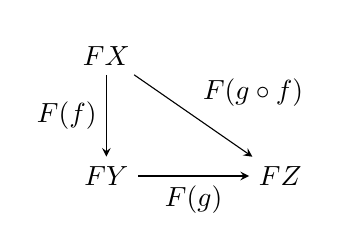
\begin{tikzpicture}
  \matrix (m) [matrix of math nodes,row sep=3em,column sep=4em,minimum width=2em]
  {
     FX &  \\
     FY & FZ \\};
  \path[-stealth]
    (m-1-1) edge node [left] {$F(f)$} (m-2-1)
    (m-2-1) edge node [below] {$F(g)$}(m-2-2)
    (m-1-1) edge node [above right] {$F(g\circ f)$} (m-2-2);
\end{tikzpicture}
\end{center}
Si $\gr{C} = \gr{D}$, on dit que $F$ est un \il{endofoncteur}.\\\\
\gr{Exemples.} On donne quelques exemples de foncteurs utiles.\begin{itemize}
\setlength\itemsep{-0.3em}
\item L'endofoncteur des parties $P : \gr{Set} \to \gr{Set}$ associe à un ensemble $X$ l'ensemble de ses parties $P(X)$, et à une fonction $f : X \to Y$ la fonction $P(f) : P(X) \to P(Y)$ définie par $P(f)(S) = f(S)$ (il s'agit de l'image directe $\{ y \in Y \mid \exists x \in S, f(x) = y \}$).
\item D'un point de vue plus informatique, l'endofoncteur $\info{List} : \gr{Set} \to \gr{Set}$ associe à $X$ l'ensemble $\info{List}(X) = X^* = \bigcup_{n\in \N} X^n$ des listes à éléments dans $X$. Pour toute fonction $f : X \to Y$, on définit $\info{List}(f) : [x_1,...,x_n] \mapsto [f(x_1),...,f(x_n)]$.
\item Pour toute catégorie $\gr{C}$, on peut définir l'endofoncteur identité $Id_\gr{C} : \gr{C} \to \gr{C}$ par $Id_\gr{C}(X) = X$ et $Id_\gr{C}(f) = f$.
\item Soit $\gr{C}$ une catégorie et $C \in |\gr{C}|$. L'endofoncteur constant $\overline{C} : \gr{C} \to \gr{C}$ est défini par $\overline{C}(X) = C$ et $\overline{C}(f) = id_C$. (On pourrait changer la catégorie de départ en n'importe quelle autre catégorie $\gr{D}$.)
\item Soit $\U : \gr{Grp} \to \gr{Set}$ le foncteur d'oubli défini par $\U(G) = |G|$ (l'ensemble sous-jacent du groupe $G$) et $\U(f) = |f|$ (la fonction sous-jacente du morphisme de groupes $f$). Plus généralement, il y a des foncteurs d'oubli $\gr{Vect} \to \gr{Set}$, $\gr{Met} \to \gr{Set}$, $\gr{Top} \to \gr{Set}$, $\gr{Meas} \to \gr{Set}$, $\gr{Graph} \to \gr{Set}$, etc. qui associent tous à un ensemble muni d'une structure l'ensemble sous-jacent.
\end{itemize}
\begin{defi}[Fidèle, plein, pleinement fidèle]
Soit $F : \gr{C} \to \gr{D}$ un foncteur. On dira que $F$ est
\begin{itemize}
\setlength\itemsep{-0.3em}
\itemz Fidèle si pour tous $X,Y \in \gr{C}$ et $f,g : X \to Y$ tels que $f \neq g$, on a $F(f) \neq F(g)$.
\itemz Plein si pour tous $X,Y \in \gr{C}$ et $\tilde{f} : F(X) \to F(Y)$, il existe $f : X \to Y$ tel que $\tilde{f} = F(f)$.
\itemz Pleinement fidèle s'il est plein et fidèle.
\end{itemize}
\end{defi}
\begin{defi}[Catégorie concrète]
Une catégorie $\gr{C}$ est concrète si elle est équipée d'un foncteur fidèle $\U : \gr{C} \to \gr{Set}$, appelé foncteur d'oubli.
\end{defi}
\gr{Exemples plus avancés de catégories.}
\begin{itemize}
\item La catégorie des petites catégories est notée $\gr{Cat}$. Ses objets sont les catégories $\gr{C}$ pour lesquelles $O(\gr{C})$ ainsi que les $\gr{C}(X,Y)$ sont des ensembles. Ses morphismes sont les foncteurs entre petites catégories, et la composition est la composition des foncteurs.
\item Pour une catégorie $\gr{C}$, la catégorie opposée $\gr{C}^{op}$ a les mêmes objets que $\gr{C}$, mais $\gr{C}^{op}(X,Y) = \gr{C}(Y,X)$ et la composition est définie par $f^{op} \circ g^{op} = (g \circ f)^{op}$. Un foncteur contravariant $G : \gr{C} \to \gr{D}$ est un foncteur covariant $\gr{C}^{op} \to \gr{D}$ i.e. tel que $G(g \circ f) = G(f) \circ G(g)$.
\end{itemize}
On a vu qu'il existe des transformations entre catégories, nommées foncteurs. \'Evidemment, les mathématiciens se sont aussi empressés de définir des transformations entre foncteurs, appelées \il{transformations naturelles}.
\begin{defi}[Transformation naturelle]
Soit $F,G : \gr{C} \to \gr{D}$ deux foncteurs. Une transformation naturelle $\lambda : F \Rightarrow G$ consiste en la donnée, pour tout $X \in \gr{C}$, d'un morphisme $\lambda_X : F(X) \to G(X)$. Ces morphismes sont tels que pour tout $f : X \to Y$, le diagramme suivant commute :
\begin{center}
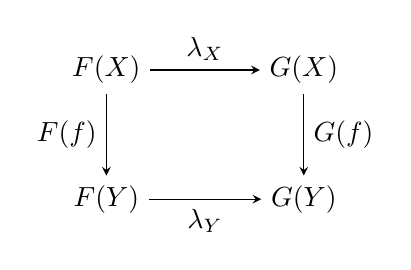
\begin{tikzpicture}
  \matrix (m) [matrix of math nodes,row sep=3em,column sep=4em,minimum width=2em]
  {
     F(X) & G(X) \\
     F(Y) & G(Y) \\};
  \path[-stealth]
    (m-1-1) edge node [above] {$\lambda_X$} (m-1-2)
    (m-1-2) edge node [right] {$G(f)$}(m-2-2)
    (m-1-1) edge node [left] {$F(f)$} (m-2-1)
    (m-2-1) edge node [below] {$\lambda_Y$}(m-2-2);
\end{tikzpicture}
\end{center}
\end{defi}
\gr{Exemples.} \begin{itemize}
\item Soit $\gr{C}$ une catégorie. La transformation naturelle identité $\mathbb{I} : Id_\gr{C} \Rightarrow Id_\gr{C}$ est définie par la donnée, pour tout objet $X \in |\gr{C}|$, du morphisme $\mathbb{I}_X = id_X$. La naturalité vient du fait que par définition de l'identité, on a pour tout $f : X \to Y$ que $id_Y \circ f = f \circ id_X$.
\item Dans $\gr{Set}$, on peut définir deux transformations naturelles élémentaires. La transformation singleton $\eta : Id_\gr{Set} \Rightarrow P$ est définie pour tout ensemble $X$ par
\begin{align*}
\eta_X : X & \to P(X) \\
x & \mapsto \{ x \}
\end{align*}
La naturalité vient du fait que $\{ f(x) \} = f(\{x\})$. La transformation union $\mu : PP \Rightarrow P$ est définie pour tout ensemble $X$ par
\begin{align*}
\mu_X : P(P(X)) & \to P(X) \\
\U & \mapsto \bigcup_{U \in \U} U
\end{align*}
La naturalité vient du fait que $\bigcup_{U\in \U} f(U) = f\left(\bigcup_{U \in \U} U\right)$. Le triplet $(P,\eta,\mu)$ vérifie en fait des conditions supplémentaires qui en font une \il{monade}, objet souvent utilisé en informatique pour modéliser des comportements branchants.
\item On peut définir une monade similaire en remplaçant les ensembles par des listes :
\begin{align*}
 \eta_X : X & \to \info{List}(X) & \mu_X : \info{List}(\info{List}(X)) & \to \info{List}(X)  \\
 x & \mapsto [x] & [[x_{1,1},...,x_{1,k_1}],...,[x_{n,1},...,x_{n,k_n}]] & \mapsto [x_{1,1},...,x_{1,k_1},...,x_{n,1},...,x_{n,k_n}]
\end{align*}
\item Intuitivement, les transformations naturelles sont des morphismes de foncteurs. Ceci est formalisé par la construction suivante. Soit $\gr{C},\gr{D}$ deux catégories, on définit la catégorie de foncteurs $\gr{D}^\gr{C}$. Ses objets sont les foncteurs $\gr{C} \to \gr{D}$ et ses morphismes sont les transformations naturelles. Les morphismes identité sont définis par $(id_F)_X = id_{FX}$, et la composition de $\alpha : F \Rightarrow G$ et $\beta : G \Rightarrow H$ est définie par $(\beta \circ \alpha)_X = \beta_X \circ \alpha_X$.
\end{itemize}
\newpage
\section{Institutions}
La théorie des institutions vient de l'observation que les différentes logiques utilisées en mathématiques ou en informatique ont une structure commune. L'étude des logiques a deux versants : la théorie des modèles et la théorie de la démonstration. En théorie de la démonstration, la définition d'une logique se fait d'un point de vue syntaxique :
\begin{itemize}
\setlength\itemsep{-0.3em}
\item[(i)] On définit ce qu'est une formule.
\item[(ii)] On définit des règles qui permettent déduire les formules les unes des autres. Par exemple, la règle du modus ponens en logique classique :
$$\infer{Q}{P & P \Rightarrow Q}$$
Parmi ces règles, certaines sont de la forme $ \frac{}{P}$ ce qui signifie que la formule $P$ est un axiome : elle est admise sans démonstration.
\end{itemize}
Une démonstration de $P$ consiste alors en un arbre de preuve représentant l'application successive des règles jusqu'à obtenir $P$. Par exemple, si on se donne comme règle le modus ponens et comme axiomes $P$ et $P \Rightarrow Q$, l'arbre suivant est une démonstration de $Q$ :
$$ \infer{Q}{\infer{P}{} & \infer{P\Rightarrow Q}{}} $$
Le point de vue de la théorie de la démonstration ne tient donc compte que des relations \il{syntaxiques} entre les formules. Le point de vue inverse, c'est-à-dire l'étude des relations \il{sémantiques}, est celui de la théorie des modèles. En théorie des modèles
\begin{itemize}
\setlength\itemsep{-0.3em}
\item[(i)] On définit ce qu'est une formule $\ph$.
\item[(ii)] On définit ce qu'est un modèle $M$.
\item[(iii)] On définit la satisfaction d'une formule par un modèle, notée $M \models \ph$.
\end{itemize}
Donnons un exemple naïf : si on prend comme formules $\ph = (\forall x, x \geq 0)$ et $\psi = (\forall x, x = 0)$, on a $\N \models \ph$ et $\N \not\models \psi$.\\\\
Une institution est la formalisation de ce qu'est une logique sous ses aspects sémantiques. La théorie des institutions est donc une sorte de généralisation de la théorie des modèles, sans grand lien avec la théorie de la démonstration.
\begin{defi}[Institution]
Une institution $\I$ est la donnée :
\begin{itemize}
\setlength\itemsep{-0.3em}
\itemz D'une catégorie $\gr{Sig}$ dont les objets sont appelés signatures et dénotés $\Sigma$.
\itemz D'un foncteur $\Sen : \gr{Sig} \to \gr{Set}$. Les éléments de $\Sen (\Sigma)$ sont appelés formules.
\itemz D'un foncteur contravariant $\Mod : \gr{Sig} \to \gr{Cat}$. Les objets et les morphismes de $\Mod(\Sigma)$ sont respectivement appelés des $\Sigma$-modèles et des $\Sigma$-morphismes.
\itemz D'une famille de relations $\models_\Sigma \subseteq \Mod(\Sigma) \times \Sen(\Sigma)$ indexée par $\gr{Sig}$, appelées relations de satisfaction, telle que la condition de satisfaction suivante est vérifiée pour tout $\sigma : \Sigma \to \Sigma'$, tout $M' \in \Mod(\Sigma')$ et tout $\ph \in \Sen(\Sigma)$ :
\begin{equation} M' \models_{\Sigma'} \Sen(\sigma)(\ph) \iff \Mod(\sigma)(M') \models_{\Sigma} \ph \label{condsat} \tag{$\ast$} \end{equation}
\end{itemize}
\end{defi}
La représentation suivante donne une idée plus claire des liens entre les différents constituants d'une institution.
\begin{center}
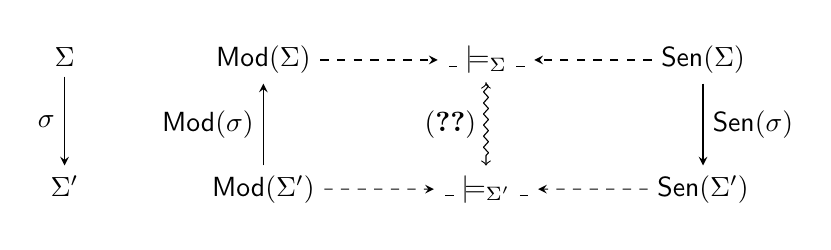
\begin{tikzpicture}
  \matrix (m) [matrix of math nodes,row sep=3em,column sep=4em,minimum width=2em]
  {
     \Sigma & \Mod(\Sigma) & \_ \models_\Sigma \_ & \Sen(\Sigma)  \\
     \Sigma' & \Mod(\Sigma') & \_ \models_{\Sigma'} \_ & \Sen(\Sigma') \\};
  \path[-stealth]
    (m-1-1) edge node [left] {$\sigma$} (m-2-1)
    (m-2-2) edge node [left] {$\Mod(\sigma)$} (m-1-2)
    (m-1-2) edge [dashed] (m-1-3)
    (m-1-4) edge [dashed] (m-1-3)
    (m-2-2) edge [dashed] (m-2-3)
    (m-2-4) edge [dashed] (m-2-3)
    (m-1-4) edge node [right] {$\Sen(\sigma)$} (m-2-4);
   \draw[<->,line join=round,
decorate, decoration={
    zigzag,
    segment length=4,
    amplitude=.9,post=lineto,
    post length=2pt
}]
    (m-1-3) -- (m-2-3) node[midway,left] {\eqref{condsat}};
\end{tikzpicture}
\end{center}
\subsection{Exemples}
On peut citer les exemples suivants d'institutions.\\\\
\gr{Logique propositionnelle ($\gr{PL}$).} L'institution $\gr{PL}$ est définie par :
\begin{itemize}
\itemz La catégorie des signatures est $\gr{Set}$. Les éléments d'un $P \in |\gr{Set}|$ seront appelées variables propositionnelles.
\itemz Le foncteur $\Sen : \gr{Set} \to \gr{Set}$ associe à $P$ l'ensemble des formules (finies) à variables dans $P$ et utilisant uniquement les connecteurs Booléens $\neg, \wedge, \vee, \Rightarrow$. Autrement dit, $\Sen(P)$ est le plus petit ensemble de formules $\Phi$ tel que
$$
\infer{p \in \Phi}{p \in P}
\qquad
\infer{\neg \ph \in \Phi}{\ph \in \Phi}
\qquad
\infer{\ph \wedge \psi \in \Phi}{\ph \in \Phi & \psi \in \Phi }
\qquad
\infer{\ph \vee \psi \in \Phi}{\ph \in \Phi & \psi \in \Phi }
\qquad
\infer{\ph \Rightarrow \psi \in \Phi}{\ph \in \Phi & \psi \in \Phi }
$$
Soit $\sigma : P \to P'$ un morphisme. Le morphisme $\Sen(\sigma)$ associe à toute formule propositionnelle $\ph \in \Sen(P)$ la formule $\Sen(\sigma)(\ph) = \ph(p \mapsto \sigma(p))$ i.e. la formule $\ph$ après renommage des variables selon $\sigma$. On peut vérifier que $\Sen$ est bien un foncteur, en effet :
\begin{align*}
 (\Sen(\sigma') \circ \Sen(\sigma)) (\ph) & = \ph(p \mapsto \sigma(p))(p' \mapsto \sigma'(p')) \\ & = \ph(p \mapsto (\sigma' \circ \sigma)(p)) \\ & = \Sen(\sigma' \circ \sigma)(\ph) 
 \end{align*}
On notera désormais $\sigma(\ph)$ pour $\Sen(\sigma)(\ph)$.
\itemz Le foncteur contravariant $\Mod : \gr{Set} \to \gr{Cat}$ associe à un ensemble $P$ le préordre $(\{0,1\}^P, \leq)$. On peut le voir comme une catégorie de la façon suivante. Ses objets sont les valuations $\nu : P \to \{0,1\}$. Lorsque $\nu \leq \nu'$ en tout point de $P$, on se donne un morphisme $\nu \to \nu'$. Par réflexivité, il y a donc des morphismes identité. La composition est $\nu \to \nu' \to \nu'' = \nu \to \nu''$, bien définie par transitivité. L'unicité de chaque morphisme $\nu \to \nu'$ donne automatiquement les conditions $(ii)$ et $(iii)$.\\\\
Soit $\sigma : P \to P'$ un morphisme. On définit $\Mod(\sigma)(\nu') = \nu' \circ \sigma$ et $\Mod(\sigma)(\nu' \to \nu'') = (\nu' \circ \sigma) \to (\nu'' \circ \sigma)$. D'abord, on doit voir que $\Mod(\sigma)$ est un foncteur de type $(\{0,1\}^{P'}, \leq) \to (\{0,1\}^P,\leq)$. On a en effet
\begin{align*} \Mod(\sigma)((\nu' \to \nu'') \circ (\nu \to \nu')) & = \Mod(\sigma)(\nu \to \nu'') = (\nu \circ \sigma) \to (\nu'' \circ \sigma) \\ & = ((\nu' \circ \sigma) \to (\nu'' \circ \sigma)) \circ ((\nu \circ \sigma) \to (\nu' \circ \sigma)) \\
& = \Mod(\sigma)(\nu' \to \nu'') \circ \Mod(\sigma)(\nu \to \nu') \end{align*}
Vérifions que $\Mod$ est bien un foncteur contravariant. Soit $\sigma : P \to P', \sigma' : P' \to P''$. Alors
\begin{align*}
(\Mod(\sigma) \circ \Mod(\sigma'))(\nu'') = \nu'' \circ \sigma' \circ \sigma = \Mod(\sigma' \circ \sigma)(\nu'')
\end{align*}
\itemz On dit que $\nu \models_P \ph$ si et seulement si la valuation $\nu$ satisfait la formule propositionnelle $\ph$ à variables dans $P$, avec la convention que $0$ et $1$ représentent respectivement le faux et le vrai. La condition de satisfaction
\begin{align*}
\nu' \models_{P'} \sigma(\ph) \iff \nu' \circ \sigma \models_P \ph 
\end{align*}
se prouve facilement par induction structurelle sur $\ph$. Une fois n'est pas coutume, on le vérifie (pour un sous-système complet de connecteurs) :
\begin{itemize}
\item Si $\ph = p$, on a $\nu' \models_{P'} \sigma(p) \iff \nu'(\sigma(p)) = 1 \iff \nu' \circ \sigma \models_P p$.
\item Si $\ph = \neg \psi$, et que le résultat est vrai pour $\psi$, on a $\nu' \models_{P'} \sigma(\ph) \iff \nu' \not\models_{P'} \sigma(\psi) \iff \nu' \circ \sigma \not\models_P \psi \iff \nu' \circ \sigma \models_P \ph$.
\item Si $\ph = \psi \wedge \theta$, et que le résultat est vrai pour $\psi$ et $\theta$, on a 
\begin{align*}
\nu' \models_{P'} \sigma(\ph) & \iff [\nu' \models_{P'} \sigma(\psi) \text{ et } \nu' \models_{P'} \sigma(\theta)] \\ & \iff [\nu' \circ \sigma \models_P \psi \text{ et } \nu' \circ \sigma \models_P \theta] \\ & \iff \nu' \circ \sigma \models_P \ph 
\end{align*}
\end{itemize}
\end{itemize}
\gr{First-order logic ($\gr{FOL}^\gr{1}$).} L'institution $\gr{FOL}^\gr{1}$ est définie par :
\begin{itemize}
\itemz On se fixe un ensemble infini de variables $\V$. La catégorie $\gr{Sig}$ a pour objets $\La = (\C, \F = \bigcup_{n\in\N^*} \F_n, \R = \bigcup_{n\in\N^*} \R_n)$ où $\C$ est un ensemble de symboles de constantes, $\F_n$ est ensemble de fonctions d'arité $n$ et $\R_n$ est un ensemble de relations d'arité $n$, aucun symbole n'étant déjà présent dans $\V$. Un morphisme de signatures $\sigma : \La \to \La'$ est constitué de trois fonctions $\C \to \C'$, $\F \to \F'$ et $\R \to \R'$ qui respectent les arités. La composition des morphismes est la composition des fonctions.
\itemz Soit une signature $\La = (\C, \F, \R)$. On définit inductivement l'ensemble des termes $\T$ comme le plus petit ensemble tel que
$$
\infer{v \in \T}{v \in \V}
\qquad
\infer{c \in \T}{c \in \C}
\qquad
\infer{f(t_1...t_n) \in \T}{f \in \F_n & t_1 \in \T & ... & t_n \in \T}
$$
L'ensemble des formules atomiques $\Phi^{at}$ est défini comme étant l'ensemble des formules de la forme $R(t_1...t_n)$ où $R \in \R_n$ et $t_1...t_n \in \T$. Le foncteur $\Sen : \gr{Sig} \to \gr{Set}$ associe à $\La$ le plus petit ensemble de formules $\Phi$ tel que
$$
\infer{\ph \in \Phi}{\ph \in \Phi^{at}}
\qquad
\infer{\neg \ph \in \Phi}{\ph \in \Phi}
\qquad
\infer{\ph \wedge \psi \in \Phi}{\ph \in \Phi & \psi \in \Phi }
\qquad
\infer{\ph \vee \psi \in \Phi}{\ph \in \Phi & \psi \in \Phi }
\qquad
\infer{\ph \Rightarrow \psi \in \Phi}{\ph \in \Phi & \psi \in \Phi }
$$
$$
\infer{\forall v \ph \in \Phi}{v \in \V & \ph \in \Phi}
\qquad
\infer{\exists v \ph \in \Phi}{v \in \V & \ph \in \Phi}
$$
Soit $\sigma : \La \to \La'$ un morphisme de signatures, alors $\Sen(\sigma)$ est le renommage selon $\sigma$, défini inductivement sur les termes par les relations $\Sen(\sigma)(v) = v$, $\Sen(\sigma)(c) = \sigma(c)$ puis $\Sen(\sigma)(f(t_1...t_n)) = \sigma(f)(\Sen(\sigma)(t_1)...\Sen(\sigma)(t_n))$ ; étendu aux formules atomiques en posant $\Sen(\sigma)(R(t_1...t_n)) = \sigma(R)(\Sen(\sigma)(t_1)...\Sen(\sigma)(t_n))$ et enfin étendu à toutes les formules. Il est facile de voir que $\Sen$ est bien un foncteur. On notera également $\sigma(\ph)$ pour $\Sen(\sigma)(\ph)$.
\itemz Le foncteur contravariant $\Mod : \gr{Sig} \to \gr{Cat}$ associe à une signature $\La = (\C, \F, \R)$ la catégorie $\Mod(\La)$ des modèles de la forme $\M = (M, \C^\M, \F^\M, \R^\M)$ constitués :
\begin{itemize}
\setlength\itemsep{-0.3em}
\item D'un ensemble $M$.
\item D'une famille d'éléments $\C^\M = (c^\M)_{c\in \C}$ où $c^\M \in M$.
\item D'une famille de fonctions $\F^\M = (f^\M)_{f \in \F}$ où $f^\M : M^n \to M$ si $f \in \F_n$.
\item D'une famille de relations $\R^\M = (R^\M)_{R \in \R}$ où $R^\M \subseteq M^n$ si $R \in \R_n$.
\end{itemize}
Un morphisme $h : \M \to \M'$ est une fonction $h : M \to M'$ telle que
\begin{enumerate}
\setlength\itemsep{-0.3em}
\item[(i)] Pour tout $c \in \C$, $h(c^\M) = c^{\M'}$.
\item[(ii)] Pour tout $f \in \F_n$ et tous $a_1...a_n \in M$, $h(f^\M(a_1...a_n)) = f^{\M'}(h(a_1)...h(a_n))$.
\item[(iii)] Pour tout $R \in \R_n$ et tous $a_1...a_n \in M$, on a $R^\M(a_1...a_n) \Rightarrow R^{\M'}(h(a_1)...h(a_n))$.
\end{enumerate}
La composition est la composition usuelle des fonctions, ce qui fait de $\Mod(\La)$ une catégorie. \`A présent, étant donné un morphisme $\sigma : \La \to \La'$, on définit $\Mod(\sigma)(\M') = \M = (M, \C^\M, \F^\M, \R^\M)$ par $M = M'$, $c^\M = \sigma(c)^{\M'}$, $f^\M = \sigma(f)^{\M'}$ et $R^\M = \sigma(R)^{\M'}$. Soit $\M_1 = \Mod(\sigma' \circ \sigma)(\M'')$ et $\M_2 = (\Mod(\sigma) \circ \Mod(\sigma'))(\M'')$. Alors $M_1 = M'' = M_2$ et pour tout $c \in \C$ on a :
\[ c^{\M_1} = (\sigma' \circ \sigma)(c)^{\M''} = \sigma'(\sigma(c))^{\M''} = \sigma(c)^{\M'} = c^{\M_2} \]
De même, on montre que $f^{\M_1} = f^{\M_2}$ et $R^{\M_1} = R^{\M_2}$, d'où $\M_1 = \M_2$.\\
On définit $\Mod(\sigma)$ sur un morphisme $h : \M \to \M'$ par $\Mod(\sigma)(h) = h$. Il s'agit bien d'un morphisme de $\Mod(\sigma)(\M) \to \Mod(\sigma)(\M')$ car $h(c^{\Mod(\sigma)(\M)}) = h(\sigma(c)^\M) = \sigma(c)^{\M'} = c^{\Mod(\sigma)(\M')}$ (et de même pour les conditions (ii) et (iii)). \\
Alors $\Mod(\sigma)$ est bien un foncteur puisque
\[ \Mod(\sigma)(g \circ h) = g \circ h = \Mod(\sigma)(g) \circ \Mod(\sigma)(h) \]
\itemz Enfin, étant donné une signature $\La$, on définit $\models_\La$ par la satisfaction usuelle du premier ordre après avoir quantifié universellement sur les variables libres. Autrement dit, si $\ph = \ph(x_1...x_n)$, on définit $\M \models_{\La} \ph$ par
$$ \forall a_1...a_n \in M^n, \M \models_\La \ph[a_1...a_n]$$
La condition de satisfaction est
$$ \M' \models_{\La'} \Sen(\sigma)(\ph) \iff \Mod(\sigma)(\M') \models_\La \ph$$
\end{itemize}
\gr{Modal Propositional Logic ($\gr{MPL}$).} L'institution $\gr{MPL}$ est définie par :
\begin{itemize}
\itemz La catégorie des signatures est $\gr{Set}$.
\itemz Le foncteur $\Sen : \gr{Set} \to \gr{Set}$ associe à une signature $P$ le plus petit ensemble de formules $\Phi$ tel que
$$
\infer{p \in \Phi}{p \in P}
\qquad
\infer{\neg \ph \in \Phi}{\ph \in \Phi}
\qquad
\infer{\ph \wedge \psi \in \Phi}{\ph \in \Phi & \psi \in \Phi }
\qquad
\infer{\ph \vee \psi \in \Phi}{\ph \in \Phi & \psi \in \Phi }
\qquad
\infer{\ph \Rightarrow \psi \in \Phi}{\ph \in \Phi & \psi \in \Phi }
$$
$$
\infer{\square \ph \in \Phi}{\ph \in P}
\qquad
\infer{\lozenge \ph \in \Phi}{\ph \in P}
$$
Le morphisme $\Sen(\sigma)$ est encore le renommage selon $\sigma$.
\itemz Pour un ensemble $P$ donné, $\Mod(P)$ a pour objets les modèles de Kripke $(I,W,R)$, qui comportent
\begin{itemize}
\setlength\itemsep{-0.3em}
\item Un ensemble d'indexation $I$.
\item Une famille $W = (W_i)_{i\in I}$ de mondes possibles, i.e., de fonctions $P \to \{ 0,1 \}$. Un monde possible peut aussi être vu comme un sous-ensemble de $P$.
\item Une relation dite d'accessibilité $R \subseteq I \times I$.
\end{itemize}
Un morphisme $h : (I,W,R) \to (I',W',R')$ de $\Mod(P)$ est une fonction $h : I \to I'$ telle que $R(i,j) \Rightarrow R'(h(i),h(j))$ et $W_i \subseteq W'_{h(i)}$ pour tout $i,j \in I$. Soit $\sigma : P \to P'$ un renommage, alors le modèle $\Mod(\sigma)((I',W',R'))$ est $(I,W,R)$ défini par $I = I'$, $R = R'$, et $W_i = W'_i \circ \sigma$ (vision fonctionnelle) ou $W_i = \{ p \mid \sigma(p) \in W'_i \}$ (vision ensembliste). Avec cette définition $\Mod$ est bien un foncteur contravariant puisque, d'une part, $(\Mod(\sigma) \circ \Mod(\sigma')) (I'',W'',R'')$ et $\Mod(\sigma' \circ \sigma)(I'',W'',R'')$ ont les mêmes $I$ et $R$, et d'autre part,
\begin{align*}
&(W''_i \circ \sigma') \circ \sigma = W''_i \circ (\sigma' \circ \sigma) &\text{ (vision fonctionnelle)}\\
&  \{ p \mid \sigma(p) \in \{ q \mid \sigma'(q) \in W''_i \}\} = \{ p \mid (\sigma' \circ \sigma)(p) \in W''_i \} & \text{ (vision ensembliste)}
\end{align*}
Il faut maintenant définir $\Mod(\sigma)$ sur un $P'$-morphisme $h : (I,(W_i)_{i\in I},R) \to (I',(W'_i)_{i\in I},R')$. On doit avoir $\Mod(\sigma)(h) : (I,(W_i \circ \sigma)_{i\in I},R) \to (I',(W'_i \circ \sigma)_{i\in I'},R)$. On pose $\Mod(\sigma)(h)(i) = h(i)$. Alors il s'agit bien d'un morphisme de modèles puisque si $R(i,j)$ on a $R(h(i),h(j))$ (car $h$ est un morphisme) d'une part, et $W_i \circ \sigma \subseteq W'_{h(i)} \circ \sigma$ (car comme $h$ est un morphisme, $W_i \subseteq W'_{h(i)}$) d'autre part. Avec cette définition, il est évident que $\Mod(\sigma)$ est un foncteur.
\itemz Soit $(I,W,R)$ un modèle de Kripke pour la signature $P$ et $i \in I$. On définit la satisfaction en $i$ par induction structurelle sur $\ph \in \Sen(P)$.
\begin{itemize}
\setlength\itemsep{-0.3em}
\item $(I,W,R) \models^i_P p$ si $p \in W_i$.
\item $(I,W,R) \models^i_P \ph \wedge \psi$ si $(I,W,R) \models^i_P \ph$ et $(I,W,R) \models^i_P \psi$.
\item $(I,W,R) \models^i_P \ph \vee \psi$ si $(I,W,R) \models^i_P \ph$ ou $(I,W,R) \models^i_P \psi$.
\item $(I,W,R) \models^i_P \neg \ph$ si $(I,W,R) \not\models^i_P \ph$.
\item $(I,W,R) \models^i_P \square \ph$ si pour tout $j$ tel que $(i,j) \in R$, $(I,W,R) \models^j_P \ph$.
\item $(I,W,R) \models^i_P \lozenge \ph$ si il existe $j$ tel que $(i,j) \in R$ et $(I,W,R) \models^j_P \ph$.
\end{itemize}
On dit enfin que $(I,W,R) \models_P \ph$ si pour tout $i \in I$, $(I,W,R) \models^i_P \ph$. Pour la dernière fois, vérifions que la relation de satisfaction est vérifiée. On se donne un morphisme $\sigma : P \to P'$ et un $P'$-modèle $(I',W',R')$. On note $(I,W,R) = \Mod(\sigma)((I',W',R'))$. On vérifie par que 
\[ (I',W',R') \models_{P'} \sigma(\ph) \iff (I,W,R) \models_P \ph \]
Pour cela, on montre d'abord par induction sur $\ph$ que pour tout $i \in I$ on a 
\begin{equation} (I',W',R') \models^i_{P'} \sigma(\ph) \iff (I,W,R) \models^i_P \ph \label{mplsat} \end{equation} 
\begin{itemize}
\setlength\itemsep{-0.3em}
\item Si $\ph = p$, pour tout $i \in I$, cela revient à dire que $\sigma(p) \in W'_i \iff p \in W_i$, vrai par définition.
\item Si $\ph = \psi \wedge \theta$, pour tout $i \in I$, cela revient à dire que 
\begin{align*} (I',W',R') \models^i_{P'} \sigma(\psi) \text{ et } (I',W',R') \models^i_{P'} \sigma(\theta) \iff (I,W,R) \models^i_P \psi \text{ et } (I,W,R) \models^i_P \theta
\end{align*}
ce qui est évident par hypothèse d'induction. Le même raisonnement est valable pour $\vee$, $\neg$ et $\Rightarrow$.
\item Si $\ph = \square \psi$, pour tout $i \in I$, on doit vérifier que
\begin{align*} & \forall j \in I' \text{ tel que } (i,j) \in R', (I',W',R') \models^j_{P'} \sigma(\psi) \\ \iff & \forall j \in I \text{ tel que } (i,j) \in R, (I,W,R) \models^j_P \psi
\end{align*}
Comme $I = I'$, $R = R'$, et que $(I',W',R') \models^j_{P'} \sigma(\psi) \iff (I,W,R) \models^j_{P} \psi$ pour tout $j \in I$ (par hypothèse d'induction), cette équivalence est vraie.
\item Si $\ph = \lozenge \psi$, on remarque que $\lozenge \psi$ et $\neg \square \neg \psi$ sont sémantiquement équivalentes et on utilise les cas précédents.
\end{itemize}
\end{itemize}
\gr{Topological MPL (TMPL)}. On abandonne le point de vue relationnel de $\gr{MPL}$ pour un point de vue topologique.
\begin{itemize}
\itemz La catégorie des signatures est $\gr{Set}$, comme dans $\gr{MPL}$.
\itemz Le foncteur $\Sen$ est le même que pour $\gr{MPL}$.
\itemz Soit $P$ un ensemble. Un objet de $\Mod(P)$ (appelé \il{topos-modèle}) est un espace topologique $(X,\tau)$ muni d'une fonction $\nu : P \to P(X)$ dite \il{de valuation}. Un morphisme $h : (X,\tau,\nu) \to (X',\tau',\nu')$ est une fonction continue telle que pour tout $p \in P$, $h(\nu(p)) \subseteq \nu'(p)$. Ceci est compatible avec les fonctions identités et la composition usuelle. Soit maintenant $\sigma : P \to P'$ et $(X',\tau',\nu')$ un $P'$-modèle. On définit le $P$-modèle $(X,\tau,\nu) = \Mod(\sigma)((X',\tau',\nu'))$ par $X = X'$, $\tau = \tau'$ et $\nu = \nu' \circ \sigma$. Pour un $P'$-morphisme $h : (X,\tau,\nu) \to (X',\tau',\nu')$, on définit le $P$-morphisme $\Mod(\sigma)(h) : (X,\tau, \nu\circ\sigma) \to (X',\tau',\nu'\circ\sigma)$ comme étant égal à $h$. Il s'agit bien d'un $P$-morphisme puisqu'il est continu (car le $P'$-morphisme $h$ est continu) et que pour tout $p \in P$, $h(\nu(\sigma(p))) \subseteq \nu'(\sigma(p))$ (d'après la propriété $h(\nu(p')) \subseteq \nu'(p')$). Il est facile de voir que $\Mod$ est un foncteur contravariant.
\itemz Comme pour $\gr{MPL}$, on dit que $(X,\tau,\nu) \models_P \ph$ lorsque $\forall x \in X, (X,\tau,\nu) \models_P^x \ph$, où l'on a défini par induction sur $\ph$ :
\begin{itemize}
\setlength\itemsep{-0.3em}
\item $(X,\tau,\nu) \models_P^x p$ si $x \in \nu(P)$.
\item $(X,\tau,\nu) \models_P^x \psi \wedge \theta$ est défini à la Tarski, comme pour $\gr{MPL}$ ; de même pour les autres connecteurs booléens.
\item $(X,\tau,\nu) \models_P^x \square \psi$ si il existe un ouvert $O \in \tau$ tel que $x \in O$ et pour tout $y \in O$, $(X,\tau,\nu) \models_P^y \psi$ (la modalité $\square$ représente \il{l'intérieur}).
\item $(X,\tau,\nu) \models_P^x \lozenge \psi$ si pour tout ouvert $O \in \tau$ tel que $x \in O$, il existe un $y \in O$ tel que $(X,\tau,\nu) \models_P^y \psi$ (la modalité $\lozenge$ représente \il{l'adhérence}).
\end{itemize}
\end{itemize}
\gr{Metric MPL (MMPL)}. Il s'agit d'une instance de $\gr{TMPL}$ dans le cas où $\tau = \tau_d$ est la topologie associée à une distance $d$.
\begin{itemize}
\itemz La catégorie des signatures est $\gr{Set}$, comme dans $\gr{MPL}$.
\itemz Le foncteur $\Sen$ le même que pour $\gr{MPL}$.
\itemz Soit $P$ un ensemble. Un objet de $\Mod(P)$ (appelé \il{modèle métrique}) est un espace métrique $(X,d)$ muni d'une fonction $\nu : P \to P(X)$ dite \il{de valuation}. Un morphisme $h : (X,d,\nu) \to (X',d',\nu')$ est une fonction continue telle que pour tout $p \in P$, $h(\nu(p)) \subseteq \nu'(p)$. Ceci est compatible avec les fonctions identités et la composition usuelle. Soit maintenant $\sigma : P \to P'$ et $(X',d',\nu')$ un $P'$-modèle. On définit le $P$-modèle $(X,d,\nu) = \Mod(\sigma)((X',d',\nu'))$ par $X = X'$, $d = d'$ et $\nu = \nu' \circ \sigma$, et le $P$-morphisme $\Mod(\sigma)(h) = h$. Il est facile de voir que $\Mod$ est un foncteur contravariant.
\itemz Comme pour $\gr{MPL}$, on dit que $(X,d,\nu) \models_P \ph$ lorsque $\forall x \in X, (X,d,\nu) \models_P^x \ph$, où l'on a défini par induction sur $\ph$ :
\begin{itemize}
\setlength\itemsep{-0.3em}
\item $(X,d,\nu) \models_P^x p$ si $x \in \nu(P)$.
\item $(X,d,\nu) \models_P^x \psi \wedge \theta$ est défini à la Tarski, comme pour $\gr{MPL}$ ; de même pour les autres connecteurs booléens.
\item $(X,d,\nu) \models_P^x \square \psi$ si il existe $\varepsilon > 0$ tel que pour tout $y$ tel que $d(x,y) < \varepsilon$, $(X,d,\nu) \models_P^y \psi$ (la modalité $\square$ représente \il{l'intérieur}).
\item $(X,\tau,\nu) \models_P^x \lozenge \psi$ si pour tout $\varepsilon > 0$ il existe un $y$ qui satisfait $d(x,y) < \varepsilon$ et $(X,d,\nu) \models_P^y \psi$ (la modalité $\lozenge$ représente \il{l'adhérence}).
\end{itemize}
\end{itemize}
\gr{Exercice.} \\ (1) Définir une institution $\gr{NMPL}$ où les modèles sont des espaces normés munis d'une valuation $(X,||-||,\nu)$. \\ (2) Définir une institution $\gr{PHMPL}$ où les modèles sont les espaces préhilbertiens munis d'une valuation $(X,\langle -, - \rangle, \nu)$. \\\\
Tout comme pour $\gr{FOL}^\gr{1}$, la définition de la relation de satisfaction dans $\gr{MPL}$, $\gr{TMPL}$ et $\gr{MMPL}$ n'est pas naturelle : l'absence de notion d'état force à quantifier universellement. On aimerait pouvoir dire \il{institutionnellement} que $\M \models_{\La} \ph[a_1...a_n]$ seulement pour certains $n$-uples $a_1...a_n$ (dans $\gr{FOL}^\gr{1}$) ou que $(I,W,R) \models_P^i \ph$ seulement pour certains mondes possibles indicés par $J \subsetneq I$ (dans $\gr{MPL}$). Ces considérations ont fait émerger la notion d'institution stratifiée.
\newpage
\section{Institutions stratifiées}
\begin{defi}[Institution stratifiée]
Une institution stratifiée $\I$ est la donnée :
\begin{itemize}
\setlength\itemsep{-0.3em}
\itemz D'une catégorie $\gr{Sig}$.
\itemz D'un foncteur $\Sen : \gr{Sig} \to \gr{Set}$.
\itemz D'un foncteur contravariant $\Mod : \gr{Sig} \to \gr{Cat}$.
\itemz D'une stratification $\lb - \rb$, c'est-à-dire la donnée : 
\begin{itemize}
\item D'une catégorie concrète $\gr{C}$ et pour tout $\Sigma \in \gr{Sig}$, d'un foncteur $\lb - \rb_\Sigma : \Mod(\Sigma) \to \gr{C}$.
\item Pour tout morphisme de signatures $\sigma : \Sigma \to \Sigma'$, d'une transformation naturelle $\lb - \rb_\sigma : \lb - \rb_{\Sigma'} \to \lb - \rb_\Sigma \circ \Mod(\sigma)$ telle que pour tout $M' \in \Mod(\Sigma')$, la fonction $\U (\lb M' \rb_\sigma) : \U ( \lb M' \rb_{\Sigma'}) \to \U (\lb \Mod(\sigma)(M') \rb_\Sigma )$ est surjective. (On omettra d'écrire le foncteur $\U$ dans la suite.)
\end{itemize}
\itemz D'une relation de satisfaction entre modèles et formules paramétrée par les états notée $M \models_\Sigma^\eta \ph$ où $\eta \in \lb M \rb_\Sigma$, telle que pour tous $\sigma : \Sigma \to \Sigma'$, $M' \in \Mod(\Sigma')$, $\eta \in \lb M' \rb_{\Sigma'}$, $\ph \in \Sen(\Sigma)$, on a l'équivalence
$$ \left(\Mod(\sigma)(M') \models_\Sigma^{\lb M' \rb_\sigma(\eta)} \ph\right) \iff \left(M' \models_{\Sigma'}^\eta \Sen(\sigma)(\ph)\right)$$
\end{itemize}
\end{defi}
\gr{Remarques.}
\begin{itemize}
\setlength\itemsep{-0.3em}
\item On peut alors définir la relation de satisfaction $\models_\Sigma \subseteq \Mod(\Sigma) \times \Sen(\Sigma)$ en disant que $M \models_\Sigma \ph$ si et seulement si $M \models_\Sigma^\eta \ph$ pour tout $\eta \in \lb M \rb_\Sigma$.
\item On notera désormais $\lb M \rb_\Sigma (\ph) = \{ \eta \in \lb M \rb_\Sigma \mid M \models_\Sigma^\eta \ph \}$. On a donc l'équivalence $M \models_\Sigma \ph \iff \lb M \rb_\Sigma (\ph) = \lb M \rb_\Sigma$.
\end{itemize}
On peut définir à partir des institutions stratifiées des notions générales de connecteurs booléens. Soit $\I$ une institution stratifiée, $\Sigma$ une signature, $M$ un $\Sigma$-modèle. Pour toute $\Sigma$-formule $\ph$, on note ici $\lb \ph \rb = \lb M \rb_\Sigma(\ph)$ et $\lb \top \rb = \lb M \rb_\Sigma$. On dira que
\begin{itemize}
\setlength\itemsep{-0.3em}
\item $\psi$ est une négation de $\ph$ si $\lb \psi \rb = \lb \top \rb \setminus \lb \ph \rb$.
\item $\psi$ est une conjonction de $\ph_1$ et $\ph_2$ si $\lb \psi \rb = \lb \ph_1 \rb \cap \lb \ph_2 \rb$.
\item $\psi$ est une disjonction de $\ph_1$ et $\ph_2$ si $\lb \psi \rb = \lb \ph_1 \rb \cup \lb \ph_2 \rb$.
\item $\psi$ est une implication de $\ph_1$ et $\ph_2$ si $\lb \psi \rb = (\lb \top \rb \setminus \lb \ph_1 \rb) \cup \lb \ph_2 \rb$.
\item $\psi$ et $\ph$ sont équivalentes, noté $\psi \equiv \ph$, si $\lb \psi \rb = \lb \ph \rb$.
\end{itemize}
On dira que l'institution $\I$ a la négation (resp. conjonction, disjonction, implication) lorsque pour tout $\Sigma \in \gr{Sig}$ et tout $\Sigma$-modèle, toute $\Sigma$-formule a une négation (resp. conjonction, disjonction, implication).
\subsection{Exemples}
\gr{Propositional Logic ($\lb \gr{PL} \rb$)}.  Soit $\1 = \{*\}$ un ensemble à un élément. On définit l'institution stratifiée $\lb \gr{PL} \rb$ en lui donnant les mêmes $\gr{Sig}$, $\Sen$, $\Mod$ que pour l'institution $\gr{PL}$. La catégorie concrète de la stratification est $\gr{Set}$. La stratification est donnée pour tout $P \in \gr{Sig}$, $\nu \in \Mod(P)$ par $\lb \nu \rb_P = \1$, et pour tout morphisme $\nu \to \nu'$ par $\lb \nu \to \nu' \rb_P = id_\1$. Il s'agit bien d'un foncteur, car si $\nu \to \nu'$ et $\nu' \to \nu''$ sont des morphismes, 
\[ \lb (\nu' \to \nu'') \circ (\nu \to \nu') \rb_P = \lb \nu \to \nu'' \rb_P = id_\1 = id_\1 \circ id_\1 = \lb \nu' \to \nu'' \rb_P \circ \lb \nu \to \nu' \rb_P \]
Pour tout $\sigma : P \to P'$, et tout $\nu \in \Mod(P')$, on définit également $\lb \nu \rb_\sigma : \lb \nu \rb_{P'} \to \lb \Mod(\sigma)(\nu) \rb_P$ par $\lb \nu \rb_\sigma =id_\1$. Pour que $\lb - \rb_\sigma$ soit une transformation naturelle, le diagramme suivant doit commuter pour tout $\nu \to \nu'$ :
\begin{center}
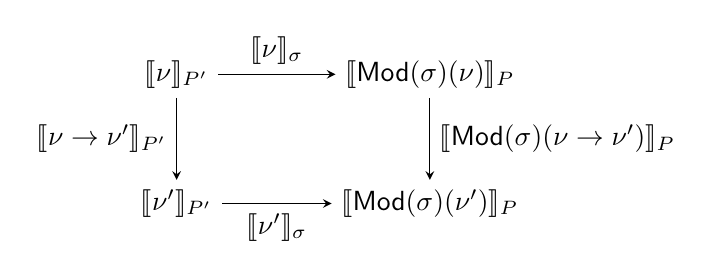
\begin{tikzpicture}
  \matrix (m) [matrix of math nodes,row sep=3em,column sep=4em,minimum width=2em]
  {
     \lb \nu \rb_{P'} & \lb \Mod(\sigma)(\nu) \rb_P \\
     \lb \nu' \rb_{P'} & \lb \Mod(\sigma)(\nu') \rb_P \\};
  \path[-stealth]
    (m-1-1) edge node [above] {$\lb \nu \rb_\sigma$} (m-1-2)
    (m-1-2) edge node [right] {$\lb \Mod(\sigma)(\nu \to \nu') \rb_P$}(m-2-2)
    (m-1-1) edge node [left] {$\lb \nu \to \nu' \rb_{P'}$} (m-2-1)
    (m-2-1) edge node [below] {$\lb \nu' \rb_\sigma$}(m-2-2);
\end{tikzpicture}
\end{center}
Dans ce cas, la commutation est triviale puisque chaque sommet est un $\1$ et chaque flèche est un $id_\1$. Pour tout $\nu \in \Mod(P')$, $\lb \nu \rb_{P'} = id_\1$ est bien surjective. La relation de satisfaction est définie par 
\[ \nu \models_P^* \ph \text{ si et seulement si } \nu \models_P \ph \]
où la relation de droite est la satisfaction usuelle pour $\gr{PL}$, et vérifie donc automatiquement la propriété de satisfaction stratifiée.\\\\\\
\gr{Modal Propositional Logic ($\lb \gr{MPL} \rb$)}. L'institution stratifiée $\lb \gr{MPL} \rb$ a les mêmes $\gr{Sig}, \Sen, \Mod$ que $\gr{MPL}$. La catégorie concrète de la stratification est $\gr{Graph}$. La stratification est donnée par
\begin{itemize}
\setlength\itemsep{-0.3em}
\itemz Pour tout $P \in \gr{Sig}$, $(I,W,R) \in \Mod(P)$, on définit $\lb (I,W,R) \rb_P = (I,R)$.
\itemz Pour tout $h : (I,W,R) \to (I',W',R')$, $\lb h \rb_P : (I,R) \to (I',R')$ est le morphisme de graphes sous-jacent à $h$. On a bien $\lb g \circ h \rb_P = \lb g \rb_P \circ \lb h \rb_P$.
\itemz Pour tout $\sigma : P \to P'$, on définit $\lb (I,W,R) \rb_\sigma = id_{(I,R)}$. Vu comme fonction, ce morphisme est bien surjectif. La commutation du diagramme se traduit par l'égalité suivante pour tout $h : (I,W,R) \to (I',W',R')$ :
\[ \lb \Mod(\sigma)(h) \rb_P \circ \lb (I,W,R) \rb_\sigma =  \lb (I',W',R') \rb_\sigma \circ \lb h \rb_{P'}\]
\[ \lb h \rb_P \circ id_{(I,R)} = id_{(I',R')} \circ \lb h \rb_{P'} \]
ce qui est vrai car vues comme fonctions $I \to I'$ cela s'écrit $h = h$.
\itemz On remarque que l'ensemble sous-jacent à $\lb (I,W,R) \rb_P$ est précisément $I$. On s'empresse donc de donner la même définition de la satisfaction $(I,W,R) \models_P^i \ph$ que dans le cas des institutions simples. On se fixe maintenant $\sigma : P \to P'$, $(I,W,R) \in \Mod(P')$, $i \in \lb (I,W,R) \rb_{P'}$, $\ph \in \Sen(\sigma)$. On doit vérifier la relation de satisfaction suivante:
\[ \Mod(\sigma)(I,W,R) \models_P^{\lb (I,W,R) \rb_\sigma (i)} \ph \iff (I,W,R) \models_{P'}^i \Sen(\sigma)(\ph)\]
qui se réécrit
\[ (I,(W_i \circ \sigma)_{i \in I}, R) \models_P^{i} \ph \iff (I,W,R) \models_{P'}^i \sigma(\ph) \]
C'est exactement ce que nous avons déjà prouvé dans le cas de $\gr{MPL}$ (équation (\ref{mplsat})).
\end{itemize}
\subsection{Liens entre institutions stratifiées et institutions}
\begin{theo}
Soit $\I$ une institution stratifiée. Alors $\I$ définit une institution.
\end{theo} 
\begin{proof}
Il n'y a rien à vérifier concernant $\gr{Sig}$, $\Sen$, $\Mod$. On se fixe $\Sigma,\Sigma' \in \gr{Sig}$, $\sigma : \Sigma \to \Sigma'$, $M' \in \Mod(\Sigma')$ et $\ph \in \Sen(\Sigma)$. On doit vérifier que
\[ \forall \eta' \in \lb M' \rb_{\Sigma'}, M' \models^{\eta'}_{\Sigma'} \Sen(\sigma)(\ph) \iff \forall \eta \in \lb \Mod(\sigma)(M') \rb_\Sigma, \Mod(\sigma)(M') \models^\eta_\Sigma \ph \] 
On utilise le fait que $M' \models_{\Sigma'}^{\eta'} \Sen(\sigma)(\ph) \iff \Mod(\sigma)(M') \models_\Sigma^{\lb M' \rb_\sigma (\eta')} \ph$. Il faut désormais montrer:
\[ \forall \eta' \in \lb M' \rb_{\Sigma'}, \Mod(\sigma)(M') \models_\Sigma^{\lb M' \rb_\sigma (\eta')} \ph \iff \forall \eta \in \lb \Mod(\sigma)(M') \rb_\Sigma, \Mod(\sigma)(M') \models^\eta_\Sigma \ph \]
Ceci est vérifié dès lors qu'on a l'égalité ensembliste 
\[ \{ \lb M' \rb_\sigma(\eta') \mid \eta' \in \lb M' \rb_{\Sigma'} \} = \lb \Mod(\sigma)(M') \rb_\Sigma \] Or, $\lb M' \rb_\sigma : \lb M' \rb_{\Sigma'} \to \lb \Mod(\sigma)(M') \rb_\Sigma$ est un morphisme surjectif (par définition d'une institution stratifiée), donc l'égalité est vraie.
\end{proof}
Il existe aussi un moyen de voir toute institution comme une institution stratifiée, via la \il{stratification interne}. Pour la définir, nous avons besoin de quelques notions auxiliaires.
\begin{defi}[Quasi-représentabilité]
Soit $\sigma : \Sigma \to \Sigma'$ un morphisme de signatures d'une institution $\I$. On dit qu'il est \il{quasi-représentable} si tout morphisme de $\Sigma'$-modèles de la forme $h : \Mod(\sigma)(M') \to N$ a une unique $\sigma$-expansion $h' : M' \to N'$, i.e., il existe un unique morphisme $h' : M' \to N'$, où $N' \in \Mod(\Sigma')$, tel que $h = \Mod(\sigma)(h')$. 
\end{defi}
\begin{defi}[Carré d'amalgamation]
Soit $\I$ une institution. Un diagramme commutatif de morphismes de signatures de la forme
\begin{center}
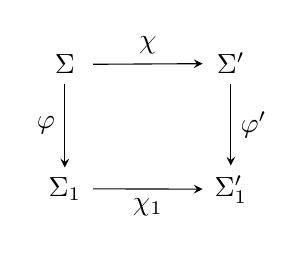
\begin{tikzpicture}
  \matrix (m) [matrix of math nodes,row sep=3em,column sep=4em,minimum width=2em]
  {
     \Sigma & \Sigma' \\
     \Sigma_1 & \Sigma'_1 \\};
  \path[-stealth]
    (m-1-1) edge node [left] {$\ph$} (m-2-1)
    (m-2-1) edge node [below] {$\chi_1$}(m-2-2)
    (m-1-1) edge node [above] {$\chi$} (m-1-2)
    (m-1-2) edge node [right] {$\ph'$} (m-2-2);
\end{tikzpicture}
\end{center}
est dit \il{carré d'amalgamation} lorsque pour tous $\Sigma'$-modèle $M'$, $\Sigma_1$-modèle $M_1$ tels que $\Mod(\chi)(M') = \Mod(\ph)(M_1)$, il existe un unique $\Sigma'_1$-modèle $M'_1$, appelé \il{amalgamation} de $M'$ et $M_1$, tel que $\Mod(\ph')(M'_1) = M'$ et $\Mod(\chi_1)(M'_1) = M_1$. On note $M'_1 = M' \otimes_{\chi,\ph} M_1$ ou encore $M'_1 = M' \otimes M_1$. Si l'unicité n'est pas garantie, on dit qu'il s'agit d'un \il{carré d'amalgamation faible}.
\end{defi}
Soit $\I = (\gr{Sig}, \Sen, \Mod, \models)$ une institution. On définit son institution stratifiée interne $St(\I) = (\gr{Sig}', \Sen', \Mod', \lb - \rb, \models)$ par :
\begin{itemize}
\itemz La catégorie $\gr{Sig}'$ a pour objets les morphismes de signatures de $\gr{Sig}$ quasi-représentables. Un morphisme de $\gr{Sig}'$ est une paire de morphismes de $\gr{Sig}$
\[ (\ph : \Sigma \to \Sigma_1, \ph' : \Sigma' \to \Sigma'_1) : (\chi : \Sigma \to \Sigma') \to (\chi_1 : \Sigma_1 \to \Sigma'_1) \] telle que la diagramme suivant est un carré d'amalgamation faible :
\begin{center}
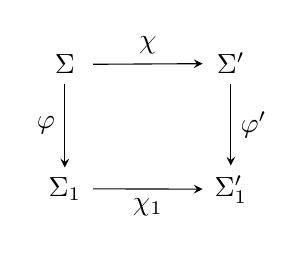
\begin{tikzpicture}
  \matrix (m) [matrix of math nodes,row sep=3em,column sep=4em,minimum width=2em]
  {
     \Sigma & \Sigma' \\
     \Sigma_1 & \Sigma'_1 \\};
  \path[-stealth]
    (m-1-1) edge node [left] {$\ph$} (m-2-1)
    (m-2-1) edge node [below] {$\chi_1$}(m-2-2)
    (m-1-1) edge node [above] {$\chi$} (m-1-2)
    (m-1-2) edge node [right] {$\ph'$} (m-2-2);
\end{tikzpicture}
\end{center}
La composition est définie par $(\psi,\psi') \circ (\ph,\ph') = (\psi \circ \ph , \psi' \circ \ph')$. On obtient bien un carré d'amalgamation faible.
\begin{center}
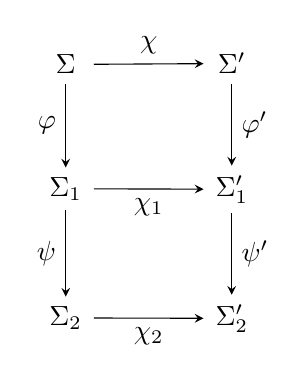
\begin{tikzpicture}
  \matrix (m) [matrix of math nodes,row sep=3em,column sep=4em,minimum width=2em]
  {
     \Sigma & \Sigma' \\
     \Sigma_1 & \Sigma'_1 \\
     \Sigma_2 & \Sigma'_2 \\};
  \path[-stealth]
    (m-1-1) edge node [left] {$\ph$} (m-2-1)
    (m-2-1) edge node [below] {$\chi_1$}(m-2-2)
    (m-1-1) edge node [above] {$\chi$} (m-1-2)
    (m-1-2) edge node [right] {$\ph'$} (m-2-2)
    (m-2-1) edge node [left] {$\psi$} (m-3-1)
    (m-3-1) edge node [below] {$\chi_2$} (m-3-2)
    (m-2-2) edge node [right] {$\psi'$} (m-3-2);
\end{tikzpicture}
\end{center}
En effet, prenons un modèle $M'$ de $\Sigma'$ et un modèle  $M_2$ de $\Sigma_2$ tels que $\Mod(\chi)(M') = \Mod(\psi \circ \ph)(M_2)$. Alors
\[ \Mod(\ph) (\Mod(\psi)(M_2)) = (\Mod(\ph) \circ \Mod(\psi))(M_2) = \Mod(\psi \circ \ph)(M_2) = \Mod(\chi)(M') \]
Le carré du haut est d'amalgamation faible, donc on obtient un modèle $M'_1$ pour $\Sigma'_1$ tel que $\Mod(\chi_1)(M'_1) = \Mod(\psi)(M_2)$ et $\Mod(\ph')(M'_1) = M'$. On peut maintenant amalgamer $M'_1$ et $M_2$. On obtient un $M'_2$ tel que $\Mod(\chi_2)(M'_2) = M_2$ et $\Mod(\psi')(M'_2) = M'_1$. Pour conclure que le grand rectangle est d'amalgamation faible, il suffit de remarquer que $\Mod(\chi_2)(M'_2) = M_2$ et $\Mod(\psi'\circ\ph')(M'_2) = \Mod(\ph')(M'_1) = M'$.\\\\
La composition dans $\gr{Sig}'$ est clairement associative, par associativité de la composition dans $\gr{Sig}$. L'identité de $(\chi : \Sigma \to \Sigma')$ est $(id_\Sigma,id_{\Sigma'})$.
\itemz Le foncteur $\Sen' : \gr{Sig} \to \gr{Set}$ est défini par
\begin{align*}
&\Sen'(\chi : \Sigma \to \Sigma') = \Sen(\Sigma') \\
&\Sen'((\ph,\ph') : \chi \to \chi_1) = \Sen(\ph') 
\end{align*}
\itemz Le foncteur contravariant $\Mod' : \gr{Sig} \to \gr{Cat}$ est défini par 
\begin{align*} 
& \Mod'((\chi : \Sigma \to \Sigma')) = \Mod(\Sigma) \\
& \Mod'((\ph,\ph') : \chi \to \chi_1) = \Mod(\ph)
\end{align*}
\itemz Pour tout $\chi : \Sigma \to \Sigma'$, le foncteur $\lb - \rb : \Mod'(\chi) \to \gr{Set}$ est défini par
\begin{align*}
& \lb M \rb_\chi = \{ M' \in \Mod(\Sigma') \mid \Mod(\chi)(M') = M \}
\end{align*}
De plus, pour tout morphisme de signatures $(\ph,\ph' : \chi \to \chi_1)$, la transformation naturelle $\lb - \rb_{(\ph,\ph')}$ est définie pour tout $M' \in \lb M \rb_{\chi_1}$ par
\[ \lb M \rb_{(\ph,\ph')}(M') = \Mod(\ph')(M') \]
\itemz Soit $\chi : \Sigma \to \Sigma'$. On définit pour tous $\ph \in \Sen'(\chi)$, $M' \in \lb M \rb_\chi$
\begin{align*}
M \models_\chi^{M'} \ph \text{ ssi } M' \models_{\Sigma'} \ph
\end{align*}
\end{itemize}


\chapter{Le théorème de \L o\'s en logique du premier ordre}
Soit $\La$ un langage du premier ordre de signature $(\C,(\F_n)_{n\in \N^*}, (\R_n)_{n\in \N^*})$, $I$ un ensemble non vide, et $(\M_i)_{i\in I}$ une famille de $\La$-structures indexées par $I$. Pour $a \in \prod_{i\in I} M_i$, on note $a(i)$ sa $i$-ème coordonnée. Pour toute $\La$-formule $\ph = \ph(x_1...x_n)$ (i.e. à variables parmi $x_1...x_n$) et tout $\bar{a} = (a_1...a_n) \in \left(\prod_{i\in I} M_i\right)^n$, on note 
\[ ||\ph(\bar{a})|| = \{ i \in I \mid \M_i \models \ph(\bar{a}(i))\} \]
où $\bar{a}(i) = a_1(i)...a_n(i)$. On a les propriétés :
\begin{itemize}
\setlength\itemsep{-0.3em}
\itemz $|| (\ph \wedge \psi) (\bar{a}) || = || \ph (\bar{a}) || \cap || \psi (\bar{a}) ||$
\itemz $|| (\ph \vee \psi) (\bar{a}) || = || \ph (\bar{a}) || \cup || \psi (\bar{a}) ||$
\itemz $|| \neg\ph (\bar{a}) || = I \setminus || \ph (\bar{a}) ||$
\end{itemize}
Le produit cartésien des $(\M_i)_{i\in I}$ est muni de la $\La$-structure suivante, notée $\M = \prod_{i\in I} \M_i$. Pour $c \in \C$, $c^\M = (c^{\M_i})_{i\in I}$. Pour $f \in \F_n$, $f^\M(a_1...a_n) = (f^{\M_i}(a_1(i)...a_n(i)))_{i\in I}$. Pour $R \in \R_n$, $R^\M = \{(a_1...a_n) \in (\prod_{i\in I} M_i)^n \mid \forall i \in I, (a_1(i)...a_n(i)) \in R^{\M_i}\}$. On a alors pour tout $\La$-terme $t = t(x_1...x_n)$ que $t^\M (a_1...a_n) = (t^{\M_i}(a_1(i)...a_n(i)))_{i\in I}$.
\section{Filtres et ultrafiltres}
\begin{defi}
Un filtre sur $I$ est une partie $\F \subseteq \mathcal{P}(I)$ qui vérifie
\begin{enumerate}
\setlength\itemsep{-0.3em}
\item[(i)] $I \in \F$, $\emptyset \notin \F$.
\item[(ii)] Si $X,Y \in \F$ alors $X \cap Y \in \F$ (stabilité par intersections finies).
\item[(iii)] Si $X \subseteq Y \subseteq I$ et $X \in \F$ alors $Y \in \F$.
\end{enumerate}
\end{defi}

\gr{Exemples.} 
\begin{itemize}
\itemz Le filtre trivial est $\F = \{ I \}$.
\itemz Le filtre engendré par $J\subseteq I$ (on dit que c'est un filtre principal) est défini par $\F_J = \{ X \in P(I) \mid J \subseteq X \}$. Si $I$ est fini, tous les filtres sont principaux (prendre un $X \in \F$ de cardinalité minimale).
\itemz Un ensemble $B \subseteq P(I)$ est une \il{base de filtre} s'il a la propriété de l'intersection finie i.e. pour tous $X_1...X_n \in B, X_1 \cap ... \cap X_n \neq \emptyset$. Dans ce cas, on pose $\F_B = \{ X \in P(I) \mid \exists n \in \N^* , \exists X_1...X_n \in B, X_1 \cap ... \cap X_n \subseteq X \}$, qui est le plus petit filtre contenant $B$. On l'appelle le filtre engendré par $B$.
\itemz Si $I$ est infini, on définit le filtre de Fréchet par $\F_\text{Fréchet} = \{ X \in P(I) \mid I\setminus X \text{ est fini}\}$. C'est un filtre qui est non principal. En effet, si $J \in \F_\text{Fréchet}$, soit $i_0 \in J$. Alors $I \setminus (J \setminus \{i_0\})$ est fini donc $J \setminus \{i_0\} \in \F_\text{Fréchet}$ d'où $\F_\text{Fréchet} \neq \F_J$.
\end{itemize}
Un \il{ultrafiltre} est un filtre maximal pour l'inclusion. Tout filtre $\F_0$ est contenu dans un ultrafiltre, par le lemme de Zorn (l'ensemble des filtres sur $I$ contenant $\F_0$ est inductif).
\begin{prop}
Soit $\F$ un filtre sur $I$. On a équivalence entre :
\begin{enumerate}
\setlength\itemsep{-0.3em}
\item[(i)] $\F$ est un ultrafiltre.
\item[(ii)] $\forall X \in P(I), X \in \F$ ou (exclusif) $I \setminus X \in \F$.
\item[(iii)] $\forall X,Y \in P(I), X \cup Y \in \F \Rightarrow X \in \F$ ou $Y \in \F$.
\item[(iv)] $\forall n \in \N^*, \forall X_1...X_n \in P(I), X_1 \cup ... \cup X_n \in \F \Rightarrow \exists i, X_i \in \F$
\end{enumerate}
\end{prop}
\preuve
Les implications $(iv) \Rightarrow (iii) \Rightarrow (ii)$ sont évidentes. Pour $(ii) \Rightarrow (i)$, on prend $X \notin \F$ (et donc $I \setminus X \in \F$), alors $\F \cup \{X\}$ n'est pas contenu dans un filtre $\F'$ sinon on aurait $\emptyset = X \cap (I\setminus X) \in \F'$. Pour $(i) \Rightarrow (iv)$, on suppose que $\F$ est un ultrafiltre et on prend $X_1...X_n \in P(I)$ tels que $\forall i, X_i \notin \F$. L'ensemble $\{ Y \cap X_i \mid Y \in \F \}$ ne peut avoir la propriété de l'intersection finie, sinon il serait la base d'un filtre contenant $\F$ et $X_i$, donc contenant strictement $\F$. Il existe donc $Y_i \in \F$ tel que $Y_i \cap X_i = \emptyset$. Alors :
\[ \left( \bigcap_{i=1}^n Y_i \right) \cap \left( \bigcup_{j=1}^n X_j \right) = \bigcup_{j=1}^n \left( \left( \bigcap_{i=1}^n Y_i \right) \cap X_j \right) = \emptyset \]
Comme $\bigcap_{i=1}^n Y_i \in \F$ on a donc $\bigcup_{j=1}^n X_j \notin \F$.
\cqfd
Les ultrafiltres principaux sont les $\F_{\{i_0\}}$ i.e. les filtres principaux engendrés par les singletons.
\begin{prop}
Soit $\U$ un ultrafiltre sur $I$. Alors $\U$ est non principal si et seulement si $\U$ contient le filtre de Fréchet.
\end{prop}
\preuve
Si $\U$ ne contient pas le filtre de Fréchet, on trouve $X \notin \U$ cofini. Alors $I \setminus X \in \U$ est fini, donc réunion finie de ses singletons : on peut trouver un $i_0 \in I \setminus X$ tel que $\{i_0\} \in \U$. On en déduit que $\U$ contient le filtre $\F_{\{i_0\}}$, maximal, donc que $\U = \F_{\{i_0\}}$. Pour la réciproque, on montre que pour un filtre principal $\F_J$, $\F_\text{Fréchet} \nsubseteq \F_J$. En effet, soit $i_0 \in J$, alors $J \cap (I \setminus \{i_0\}) = J \setminus \{i_0\} \notin \F_J$, d'où $I \setminus \{i_0\} \notin \F_J$ alors que $I \setminus \{i_0\} \in \F_\text{Fréchet}$.
\cqfd
\section{Produits réduits et ultraproduits}
Pour tout filtre $\F$ sur $I$ on définit une relation binaire sur $M = \prod_{i\in I} M_i$ par :
\begin{align*}
a \sim_\F b & \equi \{ i \in I \mid a(i) = b(i) \} \in \F \\
& (\equi || a = b || \in \F) \end{align*}
\begin{prop}
La relation $\sim_\F$ est une relation d'équivalence. De plus, pour tous $a_1...a_n,b_1...b_n \in \prod_{i\in I} M_i$, tout $f \in \F_n$ et tout $R \in \R_n$, on a :
\begin{align*}
\forall j \in \llbracket 1,n \rrbracket, a_j \sim_\F b_j \Rightarrow & f^\M (a_1...a_n) \sim_\F f^\M (b_1...b_n) \\ & \text{ et } ||R(a_1...a_n)|| \in \F \equi ||R(b_1...b_n)||\in \F
\end{align*}
\end{prop}
\preuve
La relation $\sim_\F$ est évidemment symétrique. Elle est réflexive car $I \in \F$. Elle est transitive car si $|| a = b || \in \F$ et $|| b = c || \in \F$ alors $ || a = c || \supseteq || a = b || \cap || b = c || \in \F$ donc $|| a = c || \in \F$. Supposons que $\forall j \in \llbracket 1,n \rrbracket, a_j \sim_\F b_j$. Alors :
\[ || f^\M(a_1...a_n) = f^\M(b_1...b_n) || \supseteq \bigcap_{j=1}^n || a_j = b_j || \in \F \]
donc $|| f^\M(a_1...a_n) = f^\M(b_1...b_n) || \in \F$ d'où $f^\M(a_1...a_n) \sim_\F f^\M(b_1...b_n)$. D'autre part, comme :
\[ || R(a_1...a_n) || \cap \bigcap_{j=1}^n || a_j = b_j || = || R(b_1...b_n) || \cap \bigcap_{j=1}^n || a_j = b_j || \]
on a l'équivalence $ || R(a_1...a_n) || \in \F \equi || R(b_1...b_n) || \in \F$.
\cqfd
\gr{Remarque.} On voit facilement que pour tout terme $t = t(x_1...x_n)$, si $\forall j \in \llbracket 1,n \rrbracket, a_j \sim_\F b_j$ alors $|| t^\M (a_1...a_n) = t^\M (b_1...b_n) || \in \F$.\\\\
On va maintenant munir le quotient d'une $\La$-structure. Soit $\pi : \prod_{i\in I} M_i \to \prod_{i\in I} M_i / \sim_\F$ la surjection canonique.
\begin{defi}
Le produit réduit des $(\M_i)_{i\in I}$ sur le filtre $\F$ est la $\La$-structure $\M$ suivante :
\begin{itemize}
\setlength\itemsep{-0.3em}
\itemz Son domaine est $\prod_{i\in I} M_i / \sim_\F$.
\itemz Pour tout $c \in \C$, $c^\M = \pi((c^{\M_i})_{i\in I})$.
\itemz Pour tout $f \in \F_n$, $a_1...a_n \in \prod_{i\in I} M_i$,
\[ f^\M(\pi(a_1)...\pi(a_n)) = \pi((f^{\M_i}(a_1(i)...a_n(i)))_{i\in I}) \]
\itemz Pour tout $R \in \R_n$,
\[ R^\M = \{ (\pi(a_1)...\pi(a_n)) \mid || R(a_1...a_n) || \in \F \} \]
\end{itemize}
Cette structure sera notée $\prod_{i\in I} \M_i / \F$.
\end{defi}
\gr{Remarques.} Par définition, $\pi : \prod_{i\in I} \M_i \to \prod_{i\in I} \M_i / \F$ est alors un homomorphisme. Si $\F = \{ I \}$, $\sim_\F$ est l'égalité et $\pi$ l'identité de $\prod_{i\in I} M_i$. Si $\F = \F_J$ pour un certain $\emptyset \neq J \subseteq I$, alors $\prod_{i\in I} \M_i / \F \cong \prod_{j \in J} \M_j$. En particulier, si $J = \{ i_0 \}$, $\prod_{i\in I} \M_i / \F \cong \M_{i_0}$.\\\\
On s'intéresse particulièrement au cas où $\F$ est un ultrafiltre $\U$. Dans ce cas, $\prod_{i\in I} \M_i / \U$ est appelé \il{ultraproduit}.
\begin{theo}[\L{}o\'s]
Soit $\U$ un ultrafiltre sur $I$. Pour toute $\La$-formule $\ph = \ph(x_1...x_n)$, tous $a_1...a_n \in \prod_{i\in I} M_i$, on a l'équivalence suivante :
\[ \prod_{i\in I} \M_i / \U \models \ph(\pi(a_1)...\pi(a_n)) \equi || \ph(a_1...a_n) || \in \U \]
\end{theo}
\preuve
On note $\M = \prod_{i\in I} \M_i$ et $\M^* = \M / \U$. La preuve est par récurrence sur la hauteur $h$ de $\ph$. On peut supposer que $\ph$ s'écrit uniquement à l'aide des connecteurs $\wedge$ et $\neg$ et du quantificateur $\exists$.\\\\
\underline{Si $h(\ph) = 0$}, $\ph$ est atomique donc $\ph = R(t_1...t_k)$ où $R \in \R_k$ et $t_1...t_k$ sont des termes à variables parmi $x_1...x_n$.
\begin{align*}
\M^* \models \ph(\pi(a_1)...\pi(a_n)) & \text{ ssi }
(t_1^{\M^*}(\pi(a_1)...\pi(a_n))...t_k^{\M^*}(\pi(a_1)...\pi(a_n))) \in \R^{\M^*} \\
& \text{ ssi } (\pi(t_1^\M (a_1...a_n))...\pi(t_k^\M (a_1...a_n))) \in \R^{\M^*} \\
& \text{ ssi } || R(t_1^\M(a_1...a_n)...t_k^\M(a_1...a_n)) || \in \U \\
& \text{ ssi } || \ph(a_1...a_n) || \in \U
\end{align*}
\underline{Si $h(\ph) = k+1$} et que la propriété est vraie pour tous les $h \leq k$, alors :
\begin{itemize}
\itemz $\ph = \theta \wedge \psi$, où $h(\theta) \leq k$ et $h(\psi) \leq k$. Alors :
\begin{align*}
\M^* \models \ph(\pi(a_1)...\pi(a_n)) & \text{ ssi }
\M^* \models \theta(\pi(a_1)...\pi(a_n)) \\ & \text{ et } \M^* \models \psi(\pi(a_1)...\pi(a_n)) \\
& \text{ ssi } || \theta(a_1...a_n) || \in U \text{ et } || \psi(a_1...a_n) || \in \U \\
& \text{ ssi } || \theta(a_1...a_n) || \cap || \psi(a_1...a_n) || \in \U \\
& \text{ ssi } || (\theta \wedge \psi)(a_1...a_n) || \in \U \\
& \text{ ssi } || \ph(a_1...a_n) || \in \U
\end{align*}
\itemz $\ph = \exists x_0 \psi$, où $h(\psi) = k$. Alors $\M^* \models \ph(\pi(a_1)...\pi(a_n))$ ssi il existe un $a_0 \in \prod_{i\in I} M_i$ tel que $\M^* \models \psi(\pi(a_0)...\pi(a_n))$ i.e. tel que $|| \psi(a_0...a_n)|| \in \U$. Comme $|| \ph(a_1...a_n) || \supseteq || \psi(a_0...a_n) ||$, on a $|| \psi(a_0...a_n) || \in \U \Rightarrow || \ph(a_1...a_n) || \in \U$. Réciproquement, supposons que $ || \ph(a_1...a_n) || \in \U$ et montrons qu'il existe un $a_0$ tel que $|| \psi(a_0...a_n) || \in \U$. Pour tout $i \in || \ph(a_1...a_n) ||$ il existe un $b^i \in M_i$ tel que $\M_i \models \psi(b^i,a_1(i)...a_n(i))$. On pose donc $a_0(i) = b^i$ pour tout $i \in || \ph(a_1...a_n) ||$, et on lui donne des valeurs quelconques pour les autres indices $i$. On a alors $|| \ph(a_1...a_n) || \subseteq || \psi(a_0...a_n) ||$ donc $||\psi(a_0...a_n) || \in \U$. On vient donc de prouver que $\M^* \models \ph(\pi(a_1)...\pi(a_n))$ ssi $||\ph(a_1...a_n)|| \in \U$.
\itemz $\ph = \neg \psi$, où $h(\psi) = k$. Alors, en utilisant la propriété $(ii)$ des ultrafiltres, on peut voir que :
\begin{align*}
\M^* \models \ph(\pi(a_1)...\pi(a_n)) & \text{ ssi } \M^* \not\models \psi(\pi(a_1)...\pi(a_n)) \\
& \text{ ssi } || \psi(a_1...a_n) || \notin \U \\
& \text{ ssi } I \setminus || \psi(a_1...a_n) || \in \U \\
& \text{ ssi } || \neg \psi(a_1...a_n) || \in \U \\
& \text{ ssi } || \ph(a_1...a_n) || \in \U
\end{align*}
\end{itemize}
\cqfd

%\chapter{Opérateurs duaux}

\nocite{*}
\bibliographystyle{plain}
\bibliography{biblireport}


\end{document}